\chapter{Introduction}
\label{chapter:introduction}

\section{Background}

The Third Industrial Revolution was characterized by a focus on automating repetitive and heavy tasks on the assembly lines. Still, this created a problem: whenever the manufacturers needed the robots to work in a different assembly process, they needed to be reprogrammed by an expert. The Fourth Industrial Revolution, also known as Industry 4.0, refers to the current trend of the manufacturing sector to become more intelligent and achieve greater automation. This trend takes advantage of the recent developments in artificial intelligence, the Internet of Things, and autonomous robots to pave the way for more efficient and flexible production processes. With Industry 4.0, robots are expected to be more adaptable and perform more actions without constant explicit programming.

The concept of \acf{hrc} emerges as part of Industry 4.0 and involves the research of mechanisms that allow humans and robots to work together to achieve a shared goal. Some of the most relevant topics in recent research include collision avoidance and human-aware planning of robot motions. However, to achieve true collaboration, it is not enough to react to the partner’s movements and intentions, the robot must anticipate them.

\acf{ai} has significantly evolved in the last years. With the increase of computational power, \acf{ml}, a subset of \acs{ai}, has become an increasingly promising method to deal with complex data like images and text, heavily contributing to areas such as visual perception and speech recognition. The ability of \acs{ml} models to learn from data with minimal human intervention and understand new data it has never seen before makes it a prime candidate to solve many problems in robotics and \acs{hrc} in particular.

Anticipation is a research topic in many areas, such as biology, brain studies, psychology, social sciences, artificial intelligence, and engineering. One of the most cited definitions in the last decades and across the various fields is Rosen's \cite{Rosen1985}:

\begin{displayquote}
An anticipatory system is a system containing a predictive model of itself and/or its environment, which allows it to change state at an instant in accord with the model's predictions pertaining to a later instant.
\end{displayquote}

In the field of biology, \textcite{Louie2010} claims that \textquote{Much, if not most, biological behavior is model-based ...} with the referred models being the \textquote{... internal predictive models of themselves and their environments ...}. \textcite{Poli2010} further claims that \textquote{... given that anticipatory behavior dramatically enhances the chances of survival, evolution itself may have found how to give anticipatory capacities to organisms, or to at least some of them.}. For example, an animal predicts that it will be attacked by its predator and dodges said attack to survive.

In the case of humans, \textcite{Louie2010} also stated, \textquote{We typically decide what to do now in terms of what we perceive will be the consequences of our action at some later time.} alluding to our anticipatory behavior. Therefore, human actions can result from reactive behavior when they are based on the past, from anticipatory behavior when they are based on predictions of the future, or from a mix of both.

%In particular, sports is a field where, according to \textcite{Smith2016}, \textquote{Proficiency in action anticipation is relevant in many performance contexts such as anticipating the direction of a shot (in soccer, hockey, tennis, volleyball, badminton, etc.), the deceptive movement of an opponent (in soccer, basketball, rugby, football, boxing, etc.), or the movement of a partner (in figure skating, dancing, etc.).}.

\section{Motivation}

\acl{hrc} is a research topic becoming increasingly important in modern industry, driven by the need to enhance productivity, efficiency, and safety in work environments \cite{RoblaGomez2017,Villani2018,Ajoudani2018,Matheson2019,Kumar2021,Castro2021}. The combination of human skills and robotic capabilities provides significant potential to improve the execution of complex and repetitive tasks. However, effective synchronization of actions and seamless communication between partners are open challenges that need to be further addressed \cite{Michalos2018,Papanastasiou2019,Hoffman2019}. In recent years, there has been a remarkable trend toward endowing collaborative robots with cognitive abilities, transforming them from simple automated machines into intelligent and adaptable collaborators. This shift is driven by the increasing demand for robots that can work alongside humans, understand their intentions, and actively contribute to complex tasks in dynamic environments. Collaborative cognition encompasses a range of essential abilities in order to enable robots to learn, predict, and anticipate human actions \cite{Rozo2018,Jiao2020,Castro2021}. 

In collaborative scenarios, assistive robots are designed to work alongside humans in assembly processes or maintenance operations, providing timely support in order to enhance the overall efficiency of the task. Robots can assist the human worker by delivering a component, tool, or part, by holding a part while the operator works on it, or by performing autonomously a specific sub-task. In any case, the ability of an assistive robot to anticipate the upcoming needs of a human operator plays a pivotal role in supporting efficient teamwork. By anticipating human intentions, actions, and needs, robots can proactively assist or complement human tasks, providing timely support and improving overall efficiency. 

The concept of intention anticipation is related to a double ability of robotic systems \cite{Hoffman2007,Williams2009,Huang2016,Duarte2018}. First, the ability to predict an action even before it occurs (or, before it is fully executed), by using the partial information provided up to a certain moment in time. The second ability consists of using this information to proactively plan their actions and adjust their behavior in real-time, providing smoother collaboration and minimizing potential conflicts or delays. However, achieving cognitive capabilities poses significant challenges, such as the need for robust real-time perception systems, efficient learning algorithms, and context understanding.

This anticipation ability can be achieved through distinct approaches, such as recognizing subtle cues, observing the progress of the task, or predicting human-object interactions \cite{Williams2009,Huang2015,Gorur2018,Gkioxari2018}. Different cues can contribute to the legibility of human actions according to the activity being performed. For example, eye gaze, head orientation, changes in body language, facial expressions, and even voice tone may be used to discriminate the operator's emotional state, level of engagement, and potential intentions. The source of anticipatory information may also result from monitoring the progress of the ongoing task and assessing the completion status of various sub-tasks. Therefore, the robot can anticipate the future by observing the sub-tasks performed in the past and reasoning about the future based on the structure of the complete task. Along the same line, the robot can predict the likely sequence of actions the operator is about to take by analyzing patterns of behavior and decision-making, enabling it to adjust its own actions.

This dissertation aims at the development of an anticipatory system to enhance human-robot collaboration in industrial settings under the AUGMANITY mobilizing project\footnote{AUGMANITY website: \url{https://www.augmanity.pt}}. It is inspired by a collaborative scenario in which the robot observes the actions of the human operator, makes predictions about the human’s intention, and reacts accordingly by either waiting for more observations or executing a physical action. \autoref{fig:usecase} illustrates the real workstation where the structure of a gas boiler for water heating is manually assembled. The collaborative robot’s main function would be to assist with the assembly task by placing the parts in the jig while coordinating its actions with those of the human operator who is focused on the riveting process.

\begin{figure}[ht]
\captionsetup{width=0.95\textwidth}
\centerline{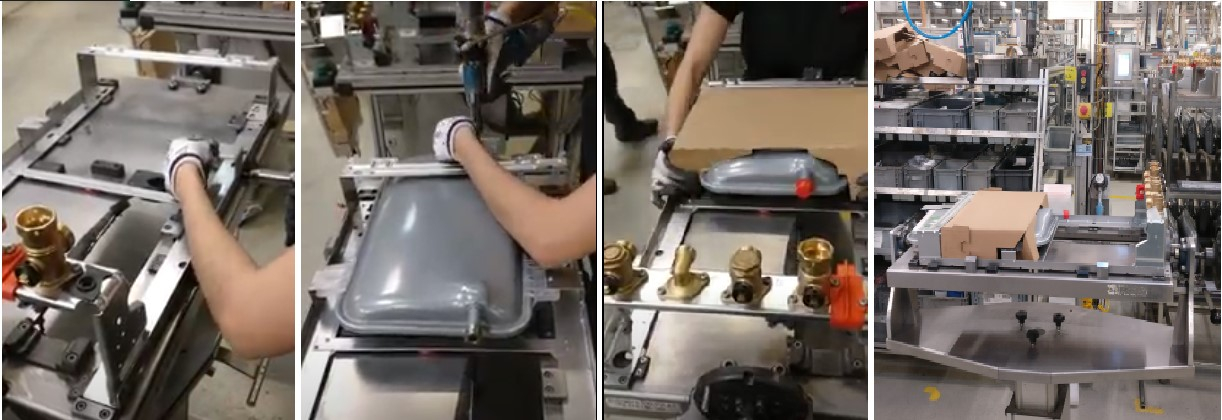
\includegraphics[width=0.95\textwidth]{figs/usecase.jpg}}
\caption{Different views of a workstation used for the manual assemblage of the structure of a gas boiler for water heating.}
\label{fig:usecase}
\end{figure}

Unlike previous approaches, this work focuses on the robot’s ability to accurately perceive and recognize the object being manipulated by the human operator as a key element in making predictions about its needs. Knowing the object in the user’s hand provides valuable contextual information revealing both current activity and future intention. A further detail that enforces the novelty of the approach is that the object is not detected directly by its shape, size, or color because, while being handled, occlusions and partial views may compromise the actual perception. Instead, the goal is to infer which object is being handled (from a list of potential objects) by the grasping pattern of the hand and fingers of the operator, as described in detail further.

The proposed concept is generic and it can be used in many \acf{hri} scenarios. The robot can use this information to adjust its posture accordingly and/or to provide relevant assistance. For example, suppose a robot is collaborating with a worker on a factory assembly line. The robot observes the worker's action and realizes he/she just picked up a specific object. Based on object recognition, the robot can adjust its own position or prepare the required tool to assist the worker in the assembly process. In this way, the robot anticipates the human's action and streamlines the workflow. This example illustrates how anticipation can be applied in \acs{hrc} scenarios to enhance interaction and overall efficiency: the robot understands the user's needs by recognizing the object being grasped or manipulated (\autoref{fig:ExperimentalSetup}).

\begin{figure}[ht]
    \captionsetup{width=0.7\textwidth}
    \centering
    {\fontsize{10}{12}\selectfont\includesvg[width=0.7\textwidth]{figs/ExpSetup.svg}}
    \caption[Illustration of a robot-assisted assembly system in a collaborative cell.]{Illustration of a robot-assisted assembly system in a collaborative cell (adapted from \cite{Malik2020}).}
    \label{fig:ExperimentalSetup}
\end{figure}

\section{Objectives}

This dissertation addresses the importance of anticipation in collaborative robotic tasks, exploring its challenges and practical applications in industry settings. The focus is on a novel framework that combines two deep learning-based models for object recognition based on the grasping posture of the user's hand during manipulation. First, the system tracks the hand manipulating an object using the MediaPipe software \cite{Lugaresi2019} that extracts 21 landmarks from an input image. Second, a multi-class classifier is trained to discriminate between four objects, taking the detected keypoints as input. The output of the deep model could be used by the robot to proactively plan its actions in real time.

In summary, the main objectives are the following:
\begin{enumerate}
    \item Review important concepts in \acs{hrc} and, in this context, study the current research direction of action anticipation including common machine learning methods and how they impact the behavior of the robot. Additionally, look into the state of the art methods related to object recognition.

    \item Establish the hardware and software tools used in this dissertation. Develop an infrastructure in \acs{ros} to support a practical implementation of action anticipation in the context of \acs{hrc} with a robot controller that considers the human partner's intentions to make appropriate decisions during the execution of a sequential assembly task.

    \item Explore and apply the potentialities of the MediaPipe framework. Produce deep learning models capable of perceiving and recognizing the objects being grasped by the user by using the right-hand keypoints. Perform extensive experiments, comparing the different models developed, to demonstrate the potential and limitations of the proposed approach analyzing, in particular, the generalization performance and/or model failure both across different trials for the same user and across multiple users.
\end{enumerate}

\section{Document Structure}

The remainder of the document is organized into four chapters. \autoref{chapter:state_of_the_art} provides an overview of the existing literature and research about collaborative robotics, action anticipation, and object recognition,  contextualizing the work within the current state of the art. \autoref{chapter:hrc_system} reviews tools used for this study and describes the initial more simple implementation of an anticipatory robot controller. \autoref{chapter:learning} presents the core components of the proposed approach, including the data acquisition process, the preprocessing steps applied to the collected data, and details of the neural network architectures implemented as multi-class classifiers and then discusses the results obtained from the experiments carried out, shedding light on the potential and limitations of the proposed approach for object recognition. \autoref{chapter:conclusion} concludes the document by outlining the main conclusions of the study and it highlights potential avenues for future research.
